\documentclass[11pt,a4paper]{article}

% =========================================================
% Core Packages
% =========================================================
\usepackage[utf8]{inputenc}
\usepackage[T1]{fontenc}
\usepackage{geometry}
\usepackage{graphicx}
\usepackage{hyperref}
\usepackage{xcolor}
\usepackage{amsmath}
\usepackage{amssymb}
\usepackage{booktabs}
\usepackage{fancyhdr}
\usepackage{tikz}
\usepackage{titlesec}
\usepackage{setspace}
\usepackage{enumitem}
\usepackage{listings}
\usepackage{tcolorbox}
\usepackage{fontawesome5}
\usepackage{multicol}
\usepackage{background}
\usepackage{tabularx}
\usepackage{colortbl}
\usepackage{calc}
\usepackage{ragged2e}
\usepackage{microtype}

% TikZ libraries
\usetikzlibrary{calc,shapes,positioning,shadows.blur,decorations.pathmorphing,backgrounds}

% tcolorbox libraries
\tcbuselibrary{skins,breakable}

% =========================================================
% Premium Typography - Palatino + Helvetica combo
% =========================================================
\usepackage{palatino}
\usepackage[scaled=0.92]{helvet}
\usepackage{inconsolata}

% =========================================================
% Page Geometry
% =========================================================
\geometry{
    a4paper,
    top=1.2in,
    bottom=1.2in,
    left=1.1in,
    right=1.1in,
    headheight=20pt
}

\setstretch{1.2}
\setlength{\parskip}{0.8em}
\setlength{\parindent}{0pt}

% Micro-typography
\microtypesetup{protrusion=true,expansion=true}

% Disable hyphenation
\hyphenpenalty=10000
\exhyphenpenalty=10000
\sloppy

% =========================================================
% Color Palette - Refined Earth Tones with Emerald Accent
% =========================================================
\definecolor{emerald}{HTML}{10B981}
\definecolor{emeraldLight}{HTML}{D1FAE5}
\definecolor{emeraldDark}{HTML}{065F46}
\definecolor{indigo}{HTML}{6366F1}
\definecolor{indigoLight}{HTML}{E0E7FF}
\definecolor{slate900}{HTML}{0F172A}
\definecolor{slate800}{HTML}{1E293B}
\definecolor{slate700}{HTML}{334155}
\definecolor{slate600}{HTML}{475569}
\definecolor{slate500}{HTML}{64748B}
\definecolor{slate400}{HTML}{94A3B8}
\definecolor{slate300}{HTML}{CBD5E1}
\definecolor{slate200}{HTML}{E2E8F0}
\definecolor{slate100}{HTML}{F1F5F9}
\definecolor{slate50}{HTML}{F8FAFC}
\definecolor{warmWhite}{HTML}{FFFBF5}
\definecolor{codeBackground}{HTML}{1E293B}
\definecolor{amber}{HTML}{F59E0B}
\definecolor{rose}{HTML}{F43F5E}

% =========================================================
% Hyperlinks
% =========================================================
\hypersetup{
    colorlinks=true,
    linkcolor=indigo,
    urlcolor=emerald,
    citecolor=slate700,
    pdfborder={0 0 0}
}

% =========================================================
% Custom Header / Footer
% =========================================================
\pagestyle{fancy}
\fancyhf{}
\renewcommand{\headrulewidth}{0pt}
\fancyhead[L]{%
    
\begin{tikzpicture}[remember picture, overlay]
        \fill[emerald] (0,0) rectangle (0.15cm,-0.5cm);
    \end{tikzpicture}%
    \hspace{0.4cm}\textcolor{slate500}{\sffamily\small\textbf{pixels.earth}}%
}
\fancyhead[R]{\textcolor{slate400}{\sffamily\small Litepaper v1.0}}
\fancyfoot[C]{%
    \textcolor{slate400}{\sffamily\small — \thepage\ —}%
}

% =========================================================
% Section Styling - Modern & Clean
% =========================================================
\titleformat{\section}
    {\sffamily\Large\bfseries\color{slate800}}
    {\colorbox{emerald}{\textcolor{white}{\sffamily\small\ \thesection\ }}}
    {0.8em}
    {}
    [\vspace{-0.3em}\textcolor{slate200}{\rule{\linewidth}{1pt}}]

\titleformat{\subsection}
    {\sffamily\large\bfseries\color{slate700}}
    {\textcolor{emerald}{\thesubsection}}
    {0.6em}
    {}

\titleformat{\subsubsection}
    {\sffamily\normalsize\bfseries\color{slate600}}
    {\textcolor{indigo}{\thesubsubsection}}
    {0.5em}
    {}

\titlespacing*{\section}{0pt}{2em}{1em}
\titlespacing*{\subsection}{0pt}{1.5em}{0.6em}
\titlespacing*{\subsubsection}{0pt}{1em}{0.4em}

% =========================================================
% Lists - Elegant Styling
% =========================================================
\setlist[itemize]{
    leftmargin=1.5em,
    label={\textcolor{emerald}{\footnotesize\faCircle}},
    itemsep=0.3em,
    parsep=0.1em
}

\setlist[enumerate]{
    leftmargin=1.8em,
    itemsep=0.3em,
    parsep=0.1em
}

\setlist[enumerate,1]{label={\textcolor{emerald}{\sffamily\bfseries\arabic*.}}}

% =========================================================
% Code Styling - Dark Theme
% =========================================================
\lstdefinestyle{darkcode}{
    backgroundcolor=\color{codeBackground},
    basicstyle=\ttfamily\small\color{slate200},
    keywordstyle=\color{emerald}\bfseries,
    stringstyle=\color{amber},
    commentstyle=\color{slate500}\itshape,
    numberstyle=\tiny\color{slate500},
    breaklines=true,
    breakatwhitespace=true,
    tabsize=4,
    showstringspaces=false,
    frame=none,
    xleftmargin=1em,
    xrightmargin=1em,
    aboveskip=0.8em,
    belowskip=0.8em,
}

\lstset{style=darkcode}

% =========================================================
% Custom Boxes
% =========================================================

% Abstract/Highlight Box
\newtcolorbox{highlightbox}{
    enhanced,
    colback=emeraldLight,
    colframe=emerald,
    boxrule=0pt,
    leftrule=4pt,
    arc=0pt,
    outer arc=0pt,
    left=16pt,
    right=16pt,
    top=14pt,
    bottom=14pt,
    fontupper=\color{slate800},
    shadow={2pt}{-2pt}{0pt}{slate300}
}

% Info Box
\newtcolorbox{infobox}{
    enhanced,
    colback=slate50,
    colframe=slate300,
    boxrule=1pt,
    arc=8pt,
    left=14pt,
    right=14pt,
    top=12pt,
    bottom=12pt,
    fontupper=\color{slate700}
}

% Code Container
\newtcolorbox{codebox}{
    enhanced,
    colback=codeBackground,
    colframe=slate700,
    boxrule=0.5pt,
    arc=6pt,
    left=0pt,
    right=0pt,
    top=0pt,
    bottom=0pt,
    boxsep=0pt,
    shadow={3pt}{-3pt}{0pt}{slate400!50}
}

% Stat Box
\newtcolorbox{statbox}[1][]{
    enhanced,
    colback=white,
    colframe=slate200,
    boxrule=1pt,
    arc=10pt,
    left=12pt,
    right=12pt,
    top=10pt,
    bottom=10pt,
    width=0.48\textwidth,
    #1
}

% =========================================================
% Custom Commands
% =========================================================

% Decorative pixel grid
\newcommand{\pixelgrid}[1]{%
    \begin{tikzpicture}[scale=#1]
        \foreach \x in {0,...,7} {
            \foreach \y in {0,...,7} {
                \pgfmathsetmacro{\hue}{mod((\x*8 + \y)*5.625 + 140, 360)}
                \definecolor{pixelcolor}{Hsb}{\hue,0.7,0.9}
                \fill[pixelcolor, rounded corners=0.02cm] 
                    (\x*0.4,\y*0.4) rectangle (\x*0.4+0.36,\y*0.4+0.36);
            }
        }
    \end{tikzpicture}%
}

% Accent line
\newcommand{\accentline}{%
    \par\vspace{0.5em}%
    \noindent\textcolor{emerald}{\rule{3cm}{2pt}}%
    \par\vspace{0.5em}%
}

% Feature item
\newcommand{\featureitem}[3]{%
    \begin{minipage}[t]{0.48\textwidth}
        \begin{tcolorbox}[
            enhanced,
            colback=white,
            colframe=slate200,
            boxrule=1pt,
            arc=10pt,
            left=12pt,
            right=12pt,
            top=12pt,
            bottom=12pt,
            height=4.5cm,
            valign=top
        ]
            \textcolor{emerald}{\Large #1}\\[0.4em]
            {\sffamily\bfseries\color{slate800}#2}\\[0.3em]
            {\small\color{slate600}#3}
        \end{tcolorbox}
    \end{minipage}%
}

% =========================================================
% Document
% =========================================================
\begin{document}

% =========================================================
% Title Page
% =========================================================
\begin{titlepage}
    
\begin{tikzpicture}[remember picture, overlay]
        % Background gradient effect
        \fill[slate900] (current page.south west) rectangle (current page.north east);
        
        % Subtle grid pattern
        \foreach \x in {-2,...,25} {
            \foreach \y in {-2,...,35} {
                \fill[slate800, opacity=0.5] (\x*0.8-2, \y*0.8-2) rectangle (\x*0.8+0.7-2, \y*0.8+0.7-2);
            }
        }
        
        % Emerald accent shapes
        \fill[emerald, opacity=0.15] (current page.north west) ++(0,-8) circle (6cm);
        \fill[indigo, opacity=0.1] (current page.south east) ++(-3,5) circle (8cm);
        
        % Top accent bar
        \fill[emerald] (current page.north west) rectangle ++(21cm,-0.4cm);
    \end{tikzpicture}
    
    \vspace*{3cm}
    
    \begin{center}
        % Logo area with pixel grid
        \pixelgrid{1.2}
        
        \vspace{1.5cm}
        
        % Main title
        {\fontsize{52}{60}\selectfont\sffamily\bfseries\textcolor{white}{pixels}\textcolor{emerald}{.earth}\par}
        
        \vspace{0.6cm}
        
        {\Large\sffamily\textcolor{slate400}{A Decentralized Earth-Scale Pixel Canvas}\par}
        
        \vspace{2cm}
        
        % Version badge
        
\begin{tikzpicture}
            \node[
                fill=emerald,
                text=white,
                rounded corners=4pt,
                inner xsep=16pt,
                inner ysep=8pt,
                font=\sffamily\bfseries
            ] {LITEPAPER v1.0};
        \end{tikzpicture}
        
        \vspace{0.5cm}
        
        {\sffamily\textcolor{slate500}{December 2025}\par}
        
        \vspace{3cm}
        
        % Tagline
        
\begin{tikzpicture}
            \node[
                text=slate300,
                font=\large\itshape
            ] {"Own a piece of the Earth. One pixel at a time."};
        \end{tikzpicture}
        
        \vfill
        
        % Tech stack badges
        \begin{tikzpicture}
            \node[
                fill=slate800,
                text=slate400,
                rounded corners=3pt,
                inner xsep=12pt,
                inner ysep=6pt,
                font=\sffamily\small
            ] (solana) {\faLink\ Built on Solana};
            
            \node[
                fill=slate800,
                text=slate400,
                rounded corners=3pt,
                inner xsep=12pt,
                inner ysep=6pt,
                font=\sffamily\small,
                right=0.5cm of solana
            ] {\faBolt\ MagicBlock Ephemeral Rollups};
        \end{tikzpicture}
        
        \vspace{1.5cm}
    \end{center}
\end{titlepage}

% =========================================================
% Abstract Page
% =========================================================
\newpage
\thispagestyle{empty}

\vspace*{1cm}

\begin{center}
    {\sffamily\LARGE\bfseries\textcolor{slate800}{Executive Summary}\par}
    \vspace{0.3cm}
    \textcolor{emerald}{\rule{4cm}{2pt}}
\end{center}

\vspace{1cm}

\begin{highlightbox}
\textbf{\sffamily\large pixels.earth} is a massively multiplayer collaborative canvas where users place colored pixels on a global Earth map. Built on Solana and accelerated by MagicBlock's Ephemeral Rollups, the platform enables real-time pixel placement with sub-second latency while preserving full on-chain security.

\vspace{0.8em}

Users can claim \textit{shards}—fixed-size pixel territories—earning passive income when others paint on their land. Through cooldowns, premium bypasses, and territory ownership, pixels.earth introduces sustainable economic incentives into collaborative digital art.
\end{highlightbox}

\vspace{1.5cm}

% Key metrics in a row
\begin{center}
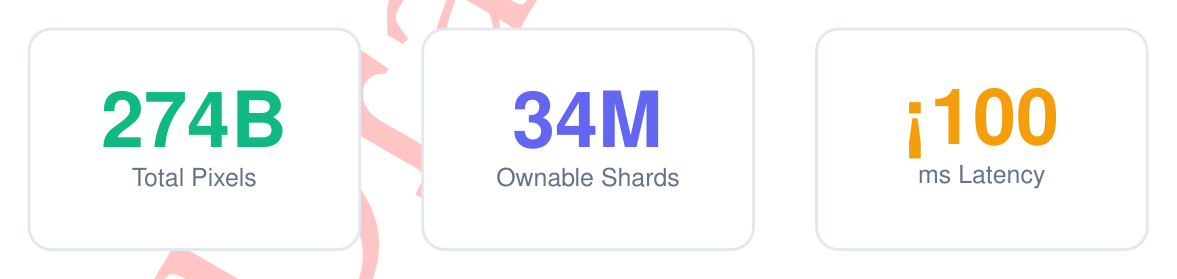
\begin{tikzpicture}
    % Metric 1
    \node[
        fill=white,
        draw=slate200,
        line width=1pt,
        rounded corners=8pt,
        minimum width=4.2cm,
        minimum height=2.8cm,
        align=center
    ] (m1) at (0,0) {
        {\fontsize{28}{32}\selectfont\sffamily\bfseries\textcolor{emerald}{274B}}\\[0.2em]
        {\small\sffamily\textcolor{slate500}{Total Pixels}}
    };
    
    % Metric 2
    \node[
        fill=white,
        draw=slate200,
        line width=1pt,
        rounded corners=8pt,
        minimum width=4.2cm,
        minimum height=2.8cm,
        align=center
    ] (m2) at (5,0) {
        {\fontsize{28}{32}\selectfont\sffamily\bfseries\textcolor{indigo}{34M}}\\[0.2em]
        {\small\sffamily\textcolor{slate500}{Ownable Shards}}
    };
    
    % Metric 3
    \node[
        fill=white,
        draw=slate200,
        line width=1pt,
        rounded corners=8pt,
        minimum width=4.2cm,
        minimum height=2.8cm,
        align=center
    ] (m3) at (10,0) {
        {\fontsize{28}{32}\selectfont\sffamily\bfseries\textcolor{amber}{<100}}\\[0.2em]
        {\small\sffamily\textcolor{slate500}{ms Latency}}
    };
\end{tikzpicture}
\end{center}

\vspace{2cm}

% Table of Contents header
\begin{center}
    {\sffamily\large\bfseries\textcolor{slate800}{Contents}\par}
    \vspace{0.3cm}
    \textcolor{slate300}{\rule{2cm}{1pt}}
\end{center}

\vspace{0.5cm}

\renewcommand{\contentsname}{}
\tableofcontents

\newpage

% =========================================================
% Section 1: Introduction
% =========================================================
\section{Introduction}

Collaborative digital art experiments—from Reddit's r/place to early blockchain pixel games—have demonstrated humanity's deep desire for collective creative expression. Yet most implementations fall short in critical ways: centralized platforms can be shut down at will, blockchain versions suffer from prohibitive latency or cost, and few provide meaningful long-term incentives for participation.

\vspace{0.5em}

\textbf{pixels.earth} addresses these fundamental challenges by unifying four essential properties:

\vspace{1em}

\noindent
\begin{minipage}[t]{0.48\textwidth}
\begin{tcolorbox}[
    enhanced,
    colback=white,
    colframe=emerald,
    boxrule=0pt,
    leftrule=3pt,
    arc=0pt,
    left=12pt,
    right=12pt,
    top=10pt,
    bottom=10pt
]
{\textcolor{emerald}{\faDatabase}\ \ \sffamily\bfseries\color{slate800}Permanent State}\\[0.3em]
{\small\color{slate600}Decentralized storage on Solana ensures artwork persists indefinitely, immune to corporate shutdowns.}
\end{tcolorbox}
\end{minipage}
\hfill
\begin{minipage}[t]{0.48\textwidth}
\begin{tcolorbox}[
    enhanced,
    colback=white,
    colframe=indigo,
    boxrule=0pt,
    leftrule=3pt,
    arc=0pt,
    left=12pt,
    right=12pt,
    top=10pt,
    bottom=10pt
]
{\textcolor{indigo}{\faBolt}\ \ \sffamily\bfseries\color{slate800}Real-Time Speed}\\[0.3em]
{\small\color{slate600}Ephemeral Rollups deliver sub-100ms interactions, matching Web2 responsiveness.}
\end{tcolorbox}
\end{minipage}

\vspace{0.8em}

\noindent
\begin{minipage}[t]{0.48\textwidth}
\begin{tcolorbox}[
    enhanced,
    colback=white,
    colframe=amber,
    boxrule=0pt,
    leftrule=3pt,
    arc=0pt,
    left=12pt,
    right=12pt,
    top=10pt,
    bottom=10pt
]
{\textcolor{amber}{\faCoins}\ \ \sffamily\bfseries\color{slate800}Sustainable Economics}\\[0.3em]
{\small\color{slate600}Territory ownership creates ongoing revenue streams, aligning creator and collector incentives.}
\end{tcolorbox}
\end{minipage}
\hfill
\begin{minipage}[t]{0.48\textwidth}
\begin{tcolorbox}[
    enhanced,
    colback=white,
    colframe=rose,
    boxrule=0pt,
    leftrule=3pt,
    arc=0pt,
    left=12pt,
    right=12pt,
    top=10pt,
    bottom=10pt
]
{\textcolor{rose}{\faGlobe}\ \ \sffamily\bfseries\color{slate800}Planetary Scale}\\[0.3em]
{\small\color{slate600}274 billion pixels mapped to Earth's surface enable truly global collaborative creation.}
\end{tcolorbox}
\end{minipage}

% =========================================================
% Section 2: Technical Architecture
% =========================================================
\section{Technical Architecture}

\subsection{Canvas Specifications}

The pixels.earth canvas maps directly onto Earth's surface using a Web Mercator projection, creating a familiar geographic context for collaborative art.

\vspace{1em}

\begin{center}
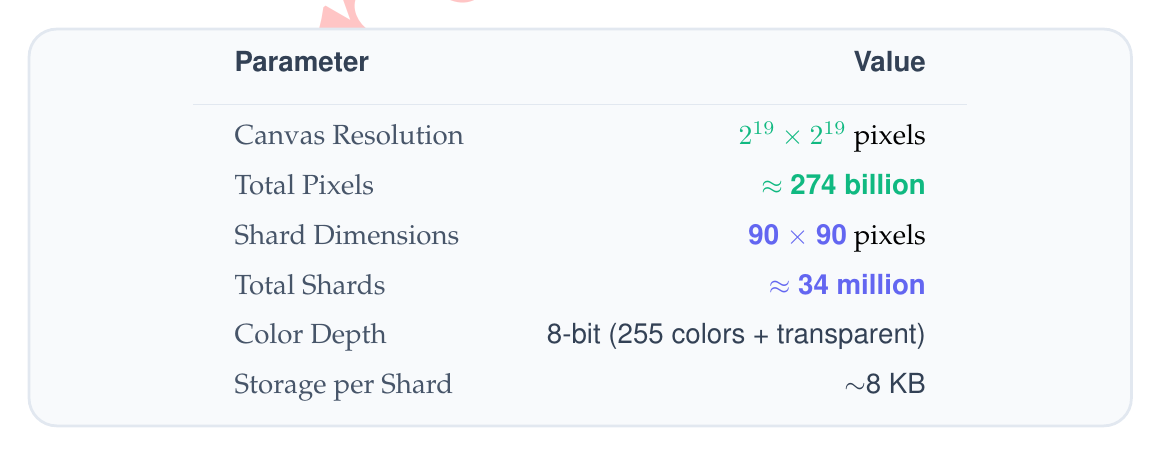
\begin{tikzpicture}
    \node[
        fill=slate50,
        draw=slate200,
        line width=1pt,
        rounded corners=10pt,
        inner sep=0pt,
        minimum width=14cm
    ] {
        \begin{tabular}{@{\hspace{1.5em}}l@{\hspace{3em}}r@{\hspace{1.5em}}}
            \\[-0.5em]
            \rowcolor{slate50}
            {\sffamily\bfseries\color{slate700}Parameter} & {\sffamily\bfseries\color{slate700}Value} \\[0.8em]
            \arrayrulecolor{slate200}\hline\\[-0.6em]
            {\color{slate600}Canvas Resolution} & {\sffamily\bfseries\color{emerald}$2^{19} \times 2^{19}$} pixels \\[0.6em]
            {\color{slate600}Total Pixels} & {\sffamily\bfseries\color{emerald}$\approx$ 274 billion} \\[0.6em]
            {\color{slate600}Shard Dimensions} & {\sffamily\bfseries\color{indigo}90 $\times$ 90} pixels \\[0.6em]
            {\color{slate600}Total Shards} & {\sffamily\bfseries\color{indigo}$\approx$ 34 million} \\[0.6em]
            {\color{slate600}Color Depth} & {\sffamily\color{slate700}8-bit (255 colors + transparent)} \\[0.6em]
            {\color{slate600}Storage per Shard} & {\sffamily\color{slate700}$\sim$8 KB} \\[0.8em]
        \end{tabular}
    };
\end{tikzpicture}
\end{center}

\subsection{Shard Architecture}

Each shard is a Solana Program Derived Address (PDA) containing pixel data and ownership metadata. This structure ensures efficient on-chain storage while enabling granular ownership.

\vspace{0.5em}

\begin{codebox}
\begin{lstlisting}[language=Rust]
pub struct PixelShard {
    pub shard_x: u16,        // X coordinate on global grid
    pub shard_y: u16,        // Y coordinate on global grid  
    pub pixels: Vec<u8>,     // 90 x 90 = 8,100 bytes
    pub creator: Pubkey,     // Original creator address
    pub bump: u8,            // PDA bump seed
}
\end{lstlisting}
\end{codebox}

\vspace{0.8em}

\begin{infobox}
\textbf{\sffamily Color Encoding:} Pixel data uses direct 8-bit indices where \texttt{0} represents transparent/erased and \texttt{1–255} map to the color palette. This compact encoding minimizes on-chain storage costs.
\end{infobox}

\subsection{Ephemeral Rollups}

MagicBlock Ephemeral Rollups enable real-time interaction while preserving the security guarantees of Solana's base layer.

\vspace{1em}

\begin{center}
\begin{tikzpicture}[
    node distance=0.8cm,
    box/.style={
        fill=white,
        draw=slate300,
        rounded corners=6pt,
        minimum width=3.2cm,
        minimum height=1.4cm,
        align=center,
        font=\small\sffamily
    },
    arrow/.style={
        ->,
        >=stealth,
        thick,
        color=emerald
    }
]
    \node[box] (init) {
        \textcolor{emerald}{\faPlay}\\[0.2em]
        \textcolor{slate700}{Initialize}\\[-0.2em]
        {\tiny\color{slate500}on Solana}
    };
    
    \node[box, right=of init] (delegate) {
        \textcolor{indigo}{\faExchangeAlt}\\[0.2em]
        \textcolor{slate700}{Delegate}\\[-0.2em]
        {\tiny\color{slate500}to Rollup}
    };
    
    \node[box, right=of delegate] (execute) {
        \textcolor{amber}{\faBolt}\\[0.2em]
        \textcolor{slate700}{Execute}\\[-0.2em]
        {\tiny\color{slate500}<100ms}
    };
    
    \node[box, right=of execute] (commit) {
        \textcolor{emerald}{\faCheck}\\[0.2em]
        \textcolor{slate700}{Commit}\\[-0.2em]
        {\tiny\color{slate500}on-chain}
    };
    
    \draw[arrow] (init) -- (delegate);
    \draw[arrow] (delegate) -- (execute);
    \draw[arrow] (execute) -- (commit);
\end{tikzpicture}
\end{center}

\vspace{0.5em}

This architecture delivers a gasless-feeling user experience while maintaining the immutability and censorship resistance of base-layer settlement.

\subsection{Session Keys}

To eliminate repeated wallet approval popups, users generate deterministic session keys derived from a single wallet signature. These keys hold a limited SOL balance and are scoped exclusively to pixel interactions, minimizing security exposure while maximizing usability.

% =========================================================
% Section 3: Game Mechanics
% =========================================================
\section{Game Mechanics}

\subsection{Territory Ownership}

Users unlock shards by paying the rent-exempt minimum on Solana. Once unlocked, ownership confers permanent rights and ongoing benefits:

\begin{itemize}
    \item \textbf{Permanent ownership} — Cannot be revoked or transferred without consent
    \item \textbf{Free painting} — Owners paint on their territory without cooldowns
    \item \textbf{Passive income} — Owners earn when others paint on their land
\end{itemize}

\subsection{Cooldown System}

Cooldowns balance accessibility with meaningful territory ownership. The system incentivizes land acquisition while keeping the canvas open to all participants.

\vspace{1em}

\begin{center}
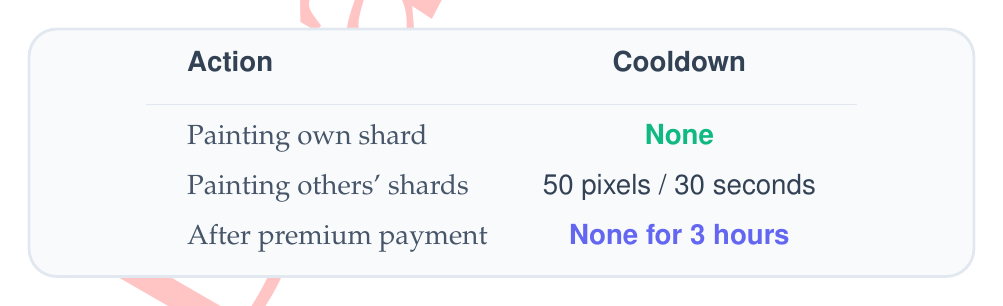
\begin{tikzpicture}
    \node[
        fill=slate50,
        draw=slate200,
        line width=1pt,
        rounded corners=10pt,
        inner sep=0pt,
        minimum width=12cm
    ] {
        \begin{tabular}{@{\hspace{1.5em}}l@{\hspace{2em}}c@{\hspace{1.5em}}}
            \\[-0.5em]
            \rowcolor{slate50}
            {\sffamily\bfseries\color{slate700}Action} & {\sffamily\bfseries\color{slate700}Cooldown} \\[0.8em]
            \arrayrulecolor{slate200}\hline\\[-0.6em]
            {\color{slate600}Painting own shard} & {\sffamily\bfseries\color{emerald}None} \\[0.6em]
            {\color{slate600}Painting others' shards} & {\sffamily\color{slate700}50 pixels / 30 seconds} \\[0.6em]
            {\color{slate600}After premium payment} & {\sffamily\bfseries\color{indigo}None for 3 hours} \\[0.8em]
        \end{tabular}
    };
\end{tikzpicture}
\end{center}

\subsection{Premium Bypass}

Premium payments flow directly to shard owners, creating a virtuous economic cycle. Artists gain unlimited creative freedom; landowners earn passive income. This alignment of incentives ensures the canvas remains both economically sustainable and creatively vibrant.

% =========================================================
% Section 4: Economic Model
% =========================================================
\section{Economic Model}

\subsection{Revenue Streams}

The platform generates sustainable revenue through three complementary mechanisms:

\begin{enumerate}
    \item \textbf{Network rent} from shard initialization (one-time, covers Solana storage)
    \item \textbf{Premium bypass payments} (ongoing, flows primarily to landowners)
    \item \textbf{Platform fee} on premium transactions (small percentage for development)
\end{enumerate}

\subsection{Token Economics}

\begin{infobox}
{\sffamily\bfseries\color{slate700}Planned:} A future governance token will enable community rewards, protocol governance, and staking mechanisms. Token design prioritizes long-term ecosystem health over short-term speculation.
\end{infobox}

% =========================================================
% Section 5: Roadmap
% =========================================================
\section{Future Roadmap}

\vspace{1em}

\begin{center}
\begin{tikzpicture}[
    phase/.style={
        fill=white,
        draw=slate200,
        line width=1pt,
        rounded corners=10pt,
        minimum width=6.5cm,
        minimum height=3.8cm,
        align=left,
        inner xsep=14pt,
        inner ysep=10pt
    }
]
    % Phase 1
    \node[phase] (p1) at (0,0) {
        {\sffamily\bfseries\large\textcolor{emerald}{Phase 1}}\\[0.1em]
        {\sffamily\small\textcolor{slate500}{Core Platform}}\\[0.6em]
        {\small\textcolor{emerald}{\faCheckCircle}\ \color{slate600}Real-time canvas}\\[0.2em]
        {\small\textcolor{emerald}{\faCheckCircle}\ \color{slate600}Shard ownership}\\[0.2em]
        {\small\textcolor{emerald}{\faCheckCircle}\ \color{slate600}Session keys}\\[0.2em]
        {\small\textcolor{emerald}{\faCheckCircle}\ \color{slate600}Mobile support}
    };
    
    % Phase 2
    \node[phase, right=0.6cm of p1] (p2) {
        {\sffamily\bfseries\large\textcolor{indigo}{Phase 2}}\\[0.1em]
        {\sffamily\small\textcolor{slate500}{Economics}}\\[0.6em]
        {\small\textcolor{slate400}{\faCircle}\ \color{slate600}Premium system}\\[0.2em]
        {\small\textcolor{slate400}{\faCircle}\ \color{slate600}Owner dashboards}\\[0.2em]
        {\small\textcolor{slate400}{\faCircle}\ \color{slate600}Leaderboards}\\[0.2em]
        {\small\textcolor{slate400}{\faCircle}\ \color{slate600}Analytics}
    };
    
    % Phase 3
    \node[phase, below=0.6cm of p1] (p3) {
        {\sffamily\bfseries\large\textcolor{amber}{Phase 3}}\\[0.1em]
        {\sffamily\small\textcolor{slate500}{Social}}\\[0.6em]
        {\small\textcolor{slate400}{\faCircle}\ \color{slate600}Faction system}\\[0.2em]
        {\small\textcolor{slate400}{\faCircle}\ \color{slate600}Territory wars}\\[0.2em]
        {\small\textcolor{slate400}{\faCircle}\ \color{slate600}User profiles}\\[0.2em]
        {\small\textcolor{slate400}{\faCircle}\ \color{slate600}Social feeds}
    };
    
    % Phase 4
    \node[phase, right=0.6cm of p3] (p4) {
        {\sffamily\bfseries\large\textcolor{rose}{Phase 4}}\\[0.1em]
        {\sffamily\small\textcolor{slate500}{Advanced}}\\[0.6em]
        {\small\textcolor{slate400}{\faCircle}\ \color{slate600}Image uploads}\\[0.2em]
        {\small\textcolor{slate400}{\faCircle}\ \color{slate600}Trading cards}\\[0.2em]
        {\small\textcolor{slate400}{\faCircle}\ \color{slate600}Cross-chain}\\[0.2em]
        {\small\textcolor{slate400}{\faCircle}\ \color{slate600}AR integration}
    };
\end{tikzpicture}
\end{center}

% =========================================================
% Section 6: Conclusion
% =========================================================
\section{Conclusion}

pixels.earth represents a new paradigm in collaborative digital art—one that merges the immediacy and accessibility of Web2 with the permanence and ownership guarantees of Web3.

By combining Solana's security with MagicBlock's Ephemeral Rollups, pixels.earth creates a living, economically sustainable canvas at planetary scale. Every pixel placed becomes part of a permanent, collectively-owned digital artifact mapped to the Earth itself.

\vspace{2cm}

\begin{center}
    \pixelgrid{0.8}
    
    \vspace{1cm}
    
    {\sffamily\LARGE\bfseries\textcolor{slate800}{pixels}\textcolor{emerald}{.earth}\par}
    
    \vspace{0.5cm}
    
    {\large\color{emerald}\url{https://pixels.earth}\par}
    
    \vspace{0.8cm}
    
    {\itshape\color{slate500}"Own a piece of the Earth. One pixel at a time."\par}
\end{center}

\end{document}
